% book example for classicthesis.sty
\documentclass[
  % Replace twoside with oneside if you are printing your thesis on a single side
  % of the paper, or for viewing on screen.
  oneside,
  %twoside,
  11pt, a4paper,
  footinclude=true,
  headinclude=true,
  cleardoublepage=empty
]{scrbook}

% To fix the usage of an old command
\DeclareOldFontCommand{\it}{\normalfont\itshape}{\mathit}

\usepackage{lipsum}
\usepackage{listings}
\usepackage[linedheaders,parts,pdfspacing,dottedtoc]{classicthesis}
\usepackage{amsmath}
\usepackage{amssymb}
\usepackage{amsthm}
\usepackage{acronym}
\usepackage[epsilon,tstt]{backnaur}
\usepackage{caption}

\usepackage[font=footnotesize]{caption}

\usepackage{chngcntr}
\counterwithin{figure}{chapter}

\usepackage{graphicx}
\graphicspath{ {Images/} }

% To setup header and footer
\clearscrheadfoot
\chead[]{\headmark}
\cfoot[\pagemark]{\pagemark}

\usepackage{xcolor}
\hypersetup{
    colorlinks=true,
    linktocpage=true,
    linkcolor={RoyalBlue},
    citecolor={RoyalBlue},
    urlcolor={RoyalBlue},
    pdftitle={Combining streaming events with static data in the Complex Event Processing tool T-Rex},
    pdfauthor={Angelo Di Pilla}
}

\lstset{
  basicstyle=\ttfamily\scriptsize,
  columns=fixed
}
\lstMakeShortInline[columns=fixed]`

\title{Combining streaming events with static data in the Complex Event Processing tool T-Rex}
\author{Angelo Di Pilla}

\begin{document}

\begin{titlepage}
    \begin{center}
        
\includegraphics[width=0.6\textwidth]{polimi_logo}\\
        \large
        Department of Industrial and Information Engineering\\
        Master degree in Computer Science and Engineering
        
        \vspace{2cm}
        
        \huge
        \textbf{Combining streaming events with static data in the Complex Event Processing tool T-Rex}
        
        \vspace{2cm}
        
        \begin{flushleft}
        \large
        \textbf{Supervisors:}\\
        Prof. Giampaolo Cugola\\
        Prof. Alessandro Margara
		\end{flushleft}
        
        \vspace{0.5cm}
        
        \begin{flushright}
        \Large
        \textbf{Thesis dissertation of:}\\
        Angelo Di Pilla (820336)
		\end{flushright}
        
        \vfill
        
        \large
        Academic year 2015 - 2016
    \end{center}
\end{titlepage}

%*******************************************************
% Abstract
%*******************************************************
\pdfbookmark[1]{Abstract}{Abstract}
\chapter*{Abstract}

\lipsum[1]

% TODO Riassunto in italiano
% %*******************************************************
% Dedication
%*******************************************************
\thispagestyle{empty}
\pdfbookmark[1]{Dedication}{Dedication}

\vspace*{3cm}

\begin{center}
    To someone special 
\end{center}

% %*******************************************************
% Acknowledgments
%*******************************************************
\pdfbookmark[1]{Acknowledgements}{acknowledgements}
\chapter*{Acknowledgements}

Put your acknowledgements here.

% %*******************************************************
% Declaration
%*******************************************************
\pdfbookmark[0]{Declaration}{declaration}
\chapter*{Declaration}
\thispagestyle{empty}

Put your declaration here.


%*******************************************************
% Table of Contents
%*******************************************************
\setcounter{tocdepth}{3} % <-- 2 includes up to subsections in the ToC
\setcounter{secnumdepth}{2} % <-- 3 numbers up to subsubsections

\tableofcontents
\addcontentsline{toc}{chapter}{\tocEntry{Table of Contents}}
\markboth{TABLE OF CONTENTS}{}

%*******************************************************
% List of Figures and of the Tables
%*******************************************************

%*******************************************************
% List of Figures
%*******************************************************    
%\pdfbookmark[1]{\listfigurename}{lof}
\listoffigures
\addcontentsline{toc}{chapter}{\tocEntry{List of Figures}}
\markboth{LIST OF FIGURES}{}

%*******************************************************
% List of Tables
%*******************************************************
%\pdfbookmark[1]{\listtablename}{lot}
%\listoftables
  
%*******************************************************
% List of Listings
%******************************************************* 
% TODO fix listings visualization
%\pdfbookmark[1]{\lstlistoflistings}{lol}
\lstlistoflistings
\addcontentsline{toc}{chapter}{\tocEntry{List of Listings}}
\markboth{LIST OF LISTINGS}{}
   
%*******************************************************
% Acronyms
%*******************************************************
%\pdfbookmark[1]{Acronyms}{acronyms}
%\chapter*{Acronyms}
%\begin{acronym}[UML]
%    \acro{DRY}{Don't Repeat Yourself}
%    \acro{API}{Application Programming Interface}
%    \acro{UML}{Unified Modeling Language}
%\end{acronym} 

% Intro
\chapter*{Introduction}
\addcontentsline{toc}{chapter}{\tocEntry{Introduction}}
\markboth{INTRODUCTION}{}


% TODO CEP background
\chapter{CEP background}
\label{chap:cep-background}

\section{Introduction}
Complex Event Processing (CEP) \cite{cep-book} consists in analysis and manipulation of streams of data, where each data item models an event occurring in an observed domain: starting from the primitive ones received as external input to the system, events are filtered, pattern matched, aggregated and combined into composite ones according to a given set of rules.

CEP represents the dual to the classical databases model, in which data are usually static or changing at a relatively slow pace and queries vary from time to time, depending on the information required at the moment. CEP instead is characterized by persistent rules applied to a continuous flow of new data.

Before stepping into more advanced topics, in this chapter I will make an overview of the field of study, from a historical contextualization to the general concepts and terminology.

\section{History and context}
The discipline was born in the '90s as an evolution of publish-subscribe systems, to satisfy the needs of expressing patterns of multiple events rather than simple topic or content filtering. From that starting point it focused on real-time applications (like IoT sensors, fraud and emergencies detection, stock markets analysis, transportation) and developed high level languages and operators to support common time related tasks.

% TODO: maybe talk about few implementation like Esper, WSO2, SQLstream and TRex

In the meantime different approaches to Information Flow Processing (IFP) \cite{ifp-survey} arose from other research fields and complemented CEP requirements and features.\\
For example the database community developed \emph{Data Stream Management Systems} (DSMSs) \cite{dsms}, which reduced everlasting streams to relational collections using windowing operators and manipulating them with continuous queries.\\
Moreover, recently \emph{distributed stream processors} started getting a lot of interest and traction from big tech companies as a new paradigm to handle extremely parallelized and throughput focused stream manipulations, in the same way \emph{Hadoop MapReduce} \cite{map-reduce} revolutionized batch processing.

Nowadays everything is slowly settling into a more unified and standardized ecosystem: tools are expanding their functionalities to match different needs of IFP and exploring the interaction with other systems and data sources.

\section{Features}
As mentioned before, CEP engines are characterized by the execution of persistent rules in low-latency applications and one of the main aspects that differentiate CEP from other similar technologies is its focus on events patterns, opposed to single events or batches.

To ease rule development and optimization, CEP engines usually define a \emph{Domain Specific Language} (DSL). These DSL are typically declarative and somehow inspired to SQL, meaning that they allow to describe the desired solution in terms of which data to retrieve and under which constraints.\\
There is a common base of operators and language constructs that can be found across most of the implementations, so let's try to review these building blocks and lay a terminology foundation for the chapters to come.

First of all it is necessary to define a sequence of events described as some kind of list of event types that have to be notified to activate the rule. That sequence is characterized by relationships of happen-before and other time constraints to delimit the eligibility to be part of the pattern. In practice, there are operators to define windows in terms of duration or number of events or delimited by the occurrence of two events that acts as boundaries.\\
In addition to temporal properties we need to apply filters based on content, so it is possible to write algebraic expressions, comparisons and possibly parameterization over the attributes of one or more events in the sequence.\\
Sometimes it is required the ability to iterate over a unknown number of events to detect a trend, some others to negate a predicate, so that the rule is fulfilled if there are no events that match the filters.\\
After a pattern is defined is important to declare selection policies, that are a way of expressing how many and which events satisfying the constraints should be picked for further processing. For example we might want to propagate only the most/least recent candidate.\\
Then we need to transform the data, combining information from multiple events or running aggregate functions.\\
Finally it may be desirable for an event notification to participate to a rule evaluation only once and then be discarded, waiting for new notifications. This practice is called event consumption and its effect and tunability can vary a lot from one implementation to another.

% TODO maybe add timers for recurring eval

% TESLA and TREX and previous work
% (Descrizione informale e citazione articoli)
\chapter{Tesla and TRex}

% TODO Introduction on previous work

\section{Tesla BNF Grammar}
% TODO add short intro

\subsection{Rule basic structure}
% TODO add short description
\begin{bnf*}
\bnfprod{rule}{
    \bnfpn{define} \bnfsp
    \bnfpn{from} \bnfsp
    \bnfpn{where} \bnfsp
    \bnfpn{consuming}
}
\end{bnf*}

\subsection{Outline of each section}
% TODO add short description
\begin{bnf*}
\bnfprod{define}{
    \bnfts{define} \bnfsp
    \bnfpn{capital identifier} \bnfsp
    \bnfts{(} \bnfsp
    \bnfpn{attributes} \bnfsp
    \bnfts{)}
}\\
\bnfprod{from}{
    \bnfts{from} \bnfsp
    \bnfpn{predicate body} \bnfsp
    \bnfpn{predicates}
}\\
\bnfprod{where}{
    \bnfts{where} \bnfsp
    \bnfpn{assignments} \bnfor
    \bnfes
}\\
\bnfprod{consuming}{
    \bnfts{consuming} \bnfsp
    \bnfpn{capital identifier} \bnfsp
    \bnfpn{capital identifiers} \bnfor
    \bnfes
}
\end{bnf*}

\subsection{Details for define}
% TODO add short description
\begin{bnf*}
\bnfprod{attributes}{
    \bnfpn{attribute} \bnfsp
    \bnfpn{attributes tail} \bnfor
    \bnfes
}\\
\bnfprod{attributes tail}{
    \bnfts{,} \bnfsp
    \bnfpn{attribute} \bnfsp
    \bnfpn{attributes tail} \bnfor
    \bnfes
}\\
\bnfprod{attribute}{
    \bnfpn{lower identifier} \bnfsp
    \bnfts{:} \bnfsp
    \bnfpn{attribute type}
}\\
\bnfprod{attribute type}{
    \bnfts{int} \bnfor
    \bnfts{float} \bnfor
    \bnfts{bool} \bnfor
    \bnfts{string}
}
\end{bnf*}

\subsection{Details for from}
% TODO add short description
\begin{bnf*}
\bnfprod{predicates}{
    \bnfts{and} \bnfsp
    \bnfpn{predicate} \bnfsp
    \bnfpn{predicates} \bnfor
    \bnfes
}\\
\bnfprod{predicate}{
    \bnfpn{event} \bnfor
    \bnfpn{aggregate}
}
\end{bnf*}

\subsection{Details for where}
% TODO add short description
\begin{bnf*}
\bnfprod{assignments}{
    \bnfpn{assignment} \bnfsp
    \bnfpn{assignments tail}
}\\
\bnfprod{assignments tail}{
    \bnfts{,} \bnfsp
    \bnfpn{assignment} \bnfsp
    \bnfpn{assignments tail} \bnfor
    \bnfes
}\\
\bnfprod{assignment}{
    \bnfpn{lower identifier} \bnfsp
    \bnfts{=} \bnfsp
    \bnfpn{expression}
}
\end{bnf*}

\subsection{Details for predicate body}
% TODO add short description
\begin{bnf*}
\bnfprod{predicate body}{
    \bnfpn{constrained tuple} \bnfsp
    \bnfpn{alias}
}\\
\bnfprod{constrained tuple}{
    \bnfpn{capital identifier} \bnfsp
    \bnfts{(} \bnfsp
    \bnfpn{constraints} \bnfsp
    \bnfts{)}
}\\
\bnfprod{constraints}{
    \bnfpn{expression} \bnfsp
    \bnfpn{constraints tail} \bnfor
    \bnfes
}\\
\bnfprod{constraints tail}{
    \bnfts{,} \bnfsp % Different from original papers!
    \bnfpn{expression} \bnfsp
    \bnfpn{constraints tail} \bnfor
    \bnfes
}\\
\bnfprod{alias}{
    \bnfts{as} \bnfsp
    \bnfpn{capital identifier} \bnfor
    \bnfes
}
\end{bnf*}

\subsection{Details for event}
% TODO add short description
\begin{bnf*}
\bnfprod{event}{
    \bnfpn{event selection} \bnfsp
    \bnfpn{predicate body} \bnfsp
    \bnfpn{timing}
}\\
\bnfprod{event selection}{
    \bnfts{each} \bnfor
    \bnfts{not} \bnfor % TODO maybe move in aggregates
    \bnfts{first} \bnfor
    \bnfts{last}
}
\end{bnf*}

\subsection{Details for aggregates}
% TODO add short description
\begin{bnf*}
\bnfprod{aggregate}{
    \bnfpn{aggregate body} \bnfsp
    \bnfpn{aggregate constraint}
}\\
\bnfprod{aggregate body}{
    \bnfpn{aggregator} \bnfsp
    \bnfts{(} \bnfsp
    \bnfpn{constrained tuple} \bnfsp
    \bnfpn{attribute selection} \bnfsp
    \bnfpn{timing} \bnfsp
    \bnfts{)}
}\\
\bnfprod{aggregator}{
    \bnfts{AVG} \bnfor
    \bnfts{SUM} \bnfor
    \bnfts{MAX} \bnfor
    \bnfts{MIN} \bnfor
    \bnfts{COUNT}
    % TODO maybe add EXISTS/ANY and NOT
}\\
\bnfprod{attribute selection}{
    \bnfts{.} \bnfsp
    \bnfpn{lower identifier} \bnfor
    \bnfes
}\\
\bnfprod{aggregate constraint}{
    \bnfpn{binary operator} \bnfsp
    \bnfpn{expression}
}
\end{bnf*}

\subsection{Details for timing}
% TODO add short description
\begin{bnf*}
\bnfprod{timing}{
    \bnfpn{within} \bnfor
    \bnfpn{between}
}\\
\bnfprod{within}{
    \bnfts{within} \bnfsp
    \bnfpn{time} \bnfsp
    \bnfts{from} \bnfsp
    \bnfpn{capital identifier}
}\\
\bnfprod{between}{
    \bnfts{between} \bnfsp
    \bnfpn{capital identifier} \bnfsp
    \bnfts{and} \bnfsp
    \bnfpn{capital identifier}
}\\
\bnfprod{time}{
    \bnfpn{float} \bnfsp
    \bnfpn{time unit} \bnfsp
}\\
\bnfprod{time unit}{
    \bnfts{d} \bnfor
    \bnfts{h} \bnfor
    \bnfts{min} \bnfor
    \bnfts{s} \bnfor
    \bnfts{ms} \bnfor
    \bnfts{us}
}
\end{bnf*}

\subsection{Details for expressions and constraints}
% TODO add short description
\begin{bnf*}
\bnfprod{expression}{
    \bnfpn{parenthesization} \bnfor
    \bnfpn{operation} \bnfor
	\bnfpn{atom}
}\\
\bnfprod{parenthesization}{
	\bnfts{(} \bnfsp
    \bnfpn{expression} \bnfsp
    \bnfts{)}
}\\
\bnfprod{operation}{
    \bnfpn{binary operation} \bnfor
    \bnfpn{unary operation}
}\\
\bnfprod{binary operation}{
    \bnfpn{expression} \bnfsp
    \bnfpn{binary operator} \bnfsp
    \bnfpn{expression}
}\\
\bnfprod{unary operation}{
    \bnfpn{unary operator} \bnfsp
    \bnfpn{expression}
}\\
\bnfprod{binary operator}{
    \bnftd{Common algebraic and comparison operators}
}\\
\bnfprod{unary operator}{
    \bnftd{Common unary operators}
}\\
\bnfprod{atom}{
    \bnfpn{identifier} \bnfor
    \bnfpn{parameter} \bnfor
    \bnfpn{immediate}
}\\
\bnfprod{identifier}{
	\bnfpn{qualifier} \bnfsp
    \bnfpn{lower identifier}
}\\
\bnfprod{qualifier}{
    \bnfpn{capital identifier} \bnfsp
    \bnfts{.} \bnfor
    \bnfes
}
\end{bnf*}

\subsection{Basic types}
% TODO add short description
\begin{bnf*}
\bnfprod{capital identifier}{
    \bnftd{An identifier starting with an uppercase letter}
}\\
\bnfprod{lower identifier}{
    \bnftd{An identifier starting with a lowercase letter}
}\\
\bnfprod{parameter}{
    \bnfts{\$} \bnfsp
    \bnfpn{lower identifier}
}\\
\bnfprod{capital identifiers}{
    \bnfts{,} \bnfsp
    \bnfpn{capital identifier} \bnfsp
    \bnfpn{capital identifiers} \bnfor
    \bnfes
}\\
\bnfprod{lower identifiers}{
    \bnfts{,} \bnfsp
    \bnfpn{lower identifier} \bnfsp
    \bnfpn{lower identifiers} \bnfor
    \bnfes
}\\
\bnfprod{immediate}{
    \bnftd{An immediate value, like a digit}
}\\
\bnfprod{float}{
    \bnftd{A floating point number}
}
\end{bnf*}

\section{Semantic}
% TODO summary of semantic as from the previous papers

\section{Ambiguities and clarifications}

During the analysis of the previously defined syntax, it appeared that there were some ambiguities and that, besides the additions of static data, a renewal of the whole language was appropriate.

\subsection{Parameters}
There is no explicit definition of the expressivity of parameterisation, meaning that it isn't clear if parameters are used in some kind of prolog like logical evaluation or they need two separate phases of assignment and usage.\\
The operating principle is indeed based on the latter option and few more issues follow from that consideration: it isn't stated that the order of definition and usage is relevant, there is no difference between assignment and comparison operators and parameters definition is mixed with selection predicates, without any syntax distinction of sort.\\
We need the new syntax to make all more clear and intuitive, reordering clauses and separating parameters definitions.

\subsection{Event declaration}
Simple events aren't declared beforehand and just appear as input of the system at runtime, that means no way of type checking them in advance against rules.\\
Complex event can be defined with different rules and possibly with different signatures, again breaking the desired type safety.\\
Impossibility of assigning a numerical id to an event type for more convenient interaction with external systems.\\
A separate declaration statement is necessary.

\subsection{Filtering}
Using the word $WHERE$ for the attributes assignment clause is ambiguous, since it wrongly reminds the $SQL$ $WHERE$ clause for filtering.\\
While the actual filtering is currently made in the $FROM$ clause, mixed with the selection predicates.\\
The idea is to change the naming and better separate selection and filtering.

\subsection{Timestamp and selection}
% TODO I'm not convinced about that, we should talk
It is not clear if timing ranges are inclusive or exclusive, while the current implementation includes the closest and excludes the furthest instant.


% Language syntax and semantic
\chapter{Language extension}

Rule basic structure
\begin{bnf*}
\bnfprod{rule}{
    \bnfpn{define} \bnfsp
    \bnfpn{from} \bnfsp
    \bnfpn{where} \bnfsp
    \bnfpn{consuming}
}
\end{bnf*}

Outline of each section
\begin{bnf*}
\bnfprod{define}{
    \bnfts{define} \bnfsp
    \bnfpn{capital identifier} \bnfsp
    \bnfts{(} \bnfsp
    \bnfpn{attributes} \bnfsp
    \bnfts{)}
}\\
\bnfprod{from}{
    \bnfts{from} \bnfsp
    \bnfpn{predicate body} \bnfsp
    \bnfpn{predicates}
}\\
\bnfprod{where}{
    \bnfts{where} \bnfsp
    \bnfpn{assignments} \bnfor
    \bnfes
}\\
\bnfprod{consuming}{
    \bnfts{consuming} \bnfsp
    \bnfpn{capital identifier} \bnfsp
    \bnfpn{capital identifiers} \bnfor
    \bnfes
}
\end{bnf*}

Details for define
\begin{bnf*}
\bnfprod{attributes}{
    \bnfpn{attribute} \bnfsp
    \bnfpn{attributes tail} \bnfor
    \bnfes
}\\
\bnfprod{attributes tail}{
    \bnfts{,} \bnfsp
    \bnfpn{attribute} \bnfsp
    \bnfpn{attributes tail} \bnfor
    \bnfes
}\\
\bnfprod{attribute}{
    \bnfpn{lower identifier} \bnfsp
    \bnfts{:} \bnfsp
    \bnfpn{attribute type}
}\\
\bnfprod{attribute type}{
    \bnfts{int} \bnfor
    \bnfts{float} \bnfor
    \bnfts{bool} \bnfor
    \bnfts{string}
}
\end{bnf*}

Details for from
\begin{bnf*}
\bnfprod{predicates}{
    \bnfts{and} \bnfsp
    \bnfpn{predicate} \bnfsp
    \bnfpn{predicates} \bnfor
    \bnfes
}\\
\bnfprod{predicate}{
    \bnfpn{event} \bnfor
    \bnfpn{aggregate} \bnfor
    \bnfpn{static}
}
\end{bnf*}

Details for where
\begin{bnf*}
\bnfprod{assignments}{
    \bnfpn{assignment} \bnfsp
    \bnfpn{assignments tail}
}\\
\bnfprod{assignments tail}{
    \bnfts{,} \bnfsp
    \bnfpn{assignment} \bnfsp
    \bnfpn{assignments tail} \bnfor
    \bnfes
}\\
\bnfprod{assignment}{
    \bnfpn{lower identifier} \bnfsp
    \bnfts{=} \bnfsp
    \bnfpn{expression}
}
\end{bnf*}

Details for predicate body
\begin{bnf*}
\bnfprod{predicate body}{
    \bnfpn{constrained tuple} \bnfsp
    \bnfpn{alias}
}\\
\bnfprod{constrained tuple}{
    \bnfpn{capital identifier} \bnfsp
    \bnfts{(} \bnfsp
    \bnfpn{constraints} \bnfsp
    \bnfts{)}
}\\
\bnfprod{constraints}{
    \bnfpn{expression} \bnfsp
    \bnfpn{constraints tail} \bnfor
    \bnfes
}\\
\bnfprod{constraints tail}{
    \bnfts{,} \bnfsp % Different from original papers!
    \bnfpn{expression} \bnfsp
    \bnfpn{constraints tail} \bnfor
    \bnfes
}\\
\bnfprod{alias}{
    \bnfts{as} \bnfsp
    \bnfpn{capital identifier} \bnfor
    \bnfes
}
\end{bnf*}

Details for event
\begin{bnf*}
\bnfprod{event}{
    \bnfpn{event selection} \bnfsp
    \bnfpn{predicate body} \bnfsp
    \bnfpn{timing}
}\\
\bnfprod{event selection}{
    \bnfts{each} \bnfor
    \bnfts{not} \bnfor
    \bnfts{first} \bnfor
    \bnfts{last}
}
\end{bnf*}

Details for aggregates
\begin{bnf*}
\bnfprod{aggregate}{
    \bnfpn{aggregate body} \bnfsp
    \bnfpn{aggregate constraint}
}\\
\bnfprod{aggregate body}{
    \bnfpn{aggregator} \bnfsp
    \bnfts{(} \bnfsp
    \bnfpn{constrained tuple} \bnfsp
    \bnfpn{timing} \bnfsp
    \bnfts{)}
}\\
\bnfprod{aggregator}{
    \bnfts{AVG} \bnfor
    \bnfts{SUM} \bnfor
    \bnfts{MAX} \bnfor
    \bnfts{MIN} \bnfor
    \bnfts{COUNT}
}\\
\bnfprod{aggregate constraint}{
    \bnfpn{binary operator} \bnfsp
    \bnfpn{expression}
}
\end{bnf*}

Details for static
\begin{bnf*}
\bnfprod{static}{
    \bnfpn{unordered static} \bnfor
    \bnfpn{ordered static}
}\\
\bnfprod{unordered static}{
    \bnfpn{unordered selection} \bnfsp
    \bnfpn{predicate body}
}\\
\bnfprod{unordered selection}{
    \bnfts{each} \bnfor
    \bnfts{any} \bnfor
    \bnfts{not}
}\\
\bnfprod{ordered static}{
    \bnfpn{ordered selection} \bnfsp
    \bnfpn{predicate body} \bnfsp
    \bnfpn{order}
}\\
\bnfprod{ordered selection}{
    \bnfts{first} \bnfor
    \bnfts{last}
}\\
\bnfprod{order}{
    \bnfts{ordered by} \bnfsp
    \bnfpn{lower identifier} \bnfsp
    \bnfpn{lower identifiers}
}
\end{bnf*}

Details for timing
\begin{bnf*}
\bnfprod{timing}{
    \bnfpn{within} \bnfor
    \bnfpn{between}
}\\
\bnfprod{within}{
    \bnfts{within} \bnfsp
    \bnfpn{time} \bnfsp
    \bnfts{from} \bnfsp
    \bnfpn{capital identifier}
}\\
\bnfprod{between}{
    \bnfts{between} \bnfsp
    \bnfpn{capital identifier} \bnfsp
    \bnfts{and} \bnfsp
    \bnfpn{capital identifier}
}\\
\bnfprod{time}{
    \bnfpn{float} \bnfsp
    \bnfpn{time unit} \bnfsp
}\\
\bnfprod{time unit}{
    \bnfts{d} \bnfor
    \bnfts{h} \bnfor
    \bnfts{min} \bnfor
    \bnfts{s} \bnfor
    \bnfts{ms} \bnfor
    \bnfts{us}
}
\end{bnf*}

Details for expressions and constraints
\begin{bnf*}
\bnfprod{expression}{
    \bnfpn{parenthesization} \bnfor
    \bnfpn{operation} \bnfor
	\bnfpn{atom}
}\\
\bnfprod{parenthesization}{
	\bnfts{(} \bnfsp
    \bnfpn{expression} \bnfsp
    \bnfts{)}
}\\
\bnfprod{operation}{
    \bnfpn{binary operation} \bnfor
    \bnfpn{unary operation}
}\\
\bnfprod{binary operation}{
    \bnfpn{expression} \bnfsp
    \bnfpn{binary operator} \bnfsp
    \bnfpn{expression}
}\\
\bnfprod{unary operation}{
    \bnfpn{unary operator} \bnfsp
    \bnfpn{expression}
}\\
\bnfprod{binary operator}{
    \bnftd{Common algebraic and comparison operators}
}\\
\bnfprod{unary operator}{
    \bnftd{Common unary operators}
}\\
\bnfprod{atom}{
    \bnfpn{identifier} \bnfor
    \bnfpn{parameter} \bnfor
    \bnfpn{immediate}
}\\
\bnfprod{identifier}{
	\bnfpn{qualifier} \bnfsp
    \bnfpn{lower identifier}
}\\
\bnfprod{qualifier}{
    \bnfpn{capital identifier} \bnfsp
    \bnfts{.} \bnfor
    \bnfes
}\\
\bnfprod{parameter}{
    \bnfts{\$} \bnfsp
    \bnfpn{lower identifier}
}\\
\bnfprod{immediate}{
    \bnftd{An immediate value, like a digit}
}
\end{bnf*}

Basic types
\begin{bnf*}
\bnfprod{capital identifier}{
    \bnftd{An identifier starting with an uppercase letter}
}\\
\bnfprod{lower identifier}{
    \bnftd{An identifier starting with a lowercase letter}
}\\
\bnfprod{capital identifiers}{
    \bnfts{,} \bnfsp
    \bnfpn{capital identifier} \bnfsp
    \bnfpn{capital identifiers} \bnfor
    \bnfes
}\\
\bnfprod{lower identifiers}{
    \bnfts{,} \bnfsp
    \bnfpn{lower identifier} \bnfsp
    \bnfpn{lower identifiers} \bnfor
    \bnfes
}\\
\bnfprod{float}{
    \bnftd{A floating point number}
}
\end{bnf*}

\begin{align*}
define &\quad CE(Att_1,\ ...\ Att_n) \\
from   &\quad SE(Att_x\ op\ Val_x)\ and \\
       &\quad each\ SD(Att_y\ op\ Val_y) \\
where  &\quad Att_1\ =\ f_1\ ...\ Att_n\ =\ f_n
\end{align*}

In the original paper have been defined the concept of $label$, to uniquely identify an event notification, the function $lab(Rule, Labels)$, to assign a label to a newly generated complex event, the trio predicate $Occurs(Type, Label)$ and the trio function $attVal(Label, Attribute)$.\\
Static data are quite similar to event notifications, so it's simple to extend the previous concepts to take them in to account.\\
We can extend labels to identify tuples too; the function $lab$ isn't changed and we can prove that the \emph{uniqueness of selection} remains valid; the predicate $Occurs$ is not relevant, since a tuple remains unchanged in every time instant; finally the function $attVal$ can be extended to return static tuple attributes.

%we can extend labels to identify them too. In this way they can concur in label generation for complex event
%To extend the language with static data, it is sufficient to say that every static tuple, event notification, is identified by a label too

\begin{align*}
&define\ CE\ from\ SE\ and\ each\ SD\ \triangleq\\
&Occurs(CE, lab(r, \{l_0, l_1\})\ \leftrightarrow\\
&(Occurs(SE, l_0)\ \wedge\ WithinP(Occurs(B, l_1),Time(l_0),x))
\end{align*}

% Abstract architecture (Drivers)
\include{Chapters/architecture}

% First implementation SQL (w/ SQLite & C++)
\chapter{Implementation}

\section{Introduction}
Given the real-time nature of a CEP engine and the extensive uptime typical of a server, a thorough implementation is of maximum importance.

In this chapter I will explain how the project is structured and how it evolved in time, highlighting the choices made to find a balance between performance and convenience.

\section{Overview}
The T-Rex project, in its entirety, is composed of the engine library, a server, a client and an HTTP proxy. The engine, written in C++ and CUDA, is the foundation of the whole system and contains the business logic and the computationally intensive tasks. The server, written in C++ as well, links the core library and provides a network interface on top of it, receiving and dispatching packets for rules and events. The client, written in Java, allows full interaction with the CEP server via TCP/IP sockets: from publish-subscribe, to rule registration, using a TESLA parser created with ANTLR. The proxy, written in JavaScript for NodeJS, exposes an HTTP interface for publishing and subscribing, but at the moment doesn't implement rule parsing and registration. For the purpose of the thesis we will focus on the library, since its is the only one relevant in terms of feasibility and performance of static data integration.

At the beginning of the collaboration the T-Rex engine was a reasonably complex and well performing piece of software, although it showed several signs of its age. It was crafted over different iterations starting from 2010 and at that time C++ was still shaped according to its 12 years old original standardization. The very next year the C++11 standard came along, beginning an incredible period of renovation for both the language and the libraries, and the adoption of these new paradigms have the potential of a great improvement of safety and extensibility.\\
In particular the broad usage of dynamically allocated objects required exceptional caution during refactoring, because any minimal oversight could lead to leaks or attempts to access freed memory. In T-Rex it was handled with manual reference counting, which is now discouraged in favor of `shared_ptr`, that uses RAII to relieve the programmer from the responsibility of updating the count.\\
Similarly a big part of the execution relied on the combination of type unions, enums and switches to describe and process TESLA expressions. The access to the wrong type or the absence of a switch case can cause bugs that aren't detected by the compiler and lead to unexpected runtime failures. In the upcoming C++17 the type \emph{variant} will be added to the standard library and it uses the power of template metaprogramming to prevent those issues at compile time.\\
Moreover threading utilities and patterns are continuously evolving and they offer new levels of abstraction that reduce the needs of synchronization and locking, improving performances and preventing data races and deadlocks.\\
In addition to those safety benefits, there are several small improvements in terms of comprehensibility: like replacing array pointers with vectors, avoiding output arguments now that compilers handle efficiently the return statement, abandoning the cumbersome naming (inherited from the C tradition) for a wise usage of namespaces, adopting foreach loops and making use of idiomatic std functions.

These innovations highlighted the weak points of the original implementation and a renewal of the code base was deemed to be a collateral requirement of the broad modifications that the library was going to face. So, after an initial attempt of progressive refactoring, I proceeded with a complete rewrite of the engine in \emph{Rust}, a new language which offers the aforementioned advantages and even more.

\section{Rust}
Rust was born around 2010 as a side project of a Mozilla engineer and later backed by the company. The first pre-alpha release was reached in 2012 and the project hit version 1.0 in May 2015. So the language is pretty young and still missing some of its planned features, but many signs suggest that it may be on the right path.\\
First of all, while in the past there were several radical changes, after they reached the release 1.0 they committed to stability and backward compatibility, adopting a well defined workflow based on reference proposals. However the project has kept evolving quickly, with a release train model over 3 months windows.\\
Moreover it has raised a lot of interest within the community and there is a strong traction from a big company, ensuring continuity. Finally it is already used in production by Mozilla itself, Dropbox and Coursera among the others.

Rust aims to be a safe and practical language for system programming, with particular attention to concurrency. Its syntax, modern and expressive, combines the best aspects of imperative, object oriented and functional programming, offering the right level of abstraction for many different task.\\
The type-system, inspired by Haskell, is based on the concept of trait, which describe a property or a behavior of an object. Traits achieve their maximum utility in combination with generics, allowing code reuse while imposing clear restrictions on the applied types.\\
Rust also implements some features typical of higher level languages, like advanced union types (enums in Rust jargon), tuples, type inference, destructuring and pattern matching.\\
However the most prominent and peculiar characteristic is its unprecedented approach to safety with the concept of data ownership. Each object is tied to a single owner at a time, ownership can be transferred via assignment, return or function arguments and the content is moved and no longer accessible from the previous variable. If we want to access data without loosing ownership, it's possible to borrow multiple immutable references or a single mutable one, in the meantime the variable is considered blocked in something conceptually similar to a read-write lock. Every reference is bounded by the lifetime of the referee and can't outlive the owner. In this way is always clear who is responsible for the resource and when the owner goes out of scope the object can be safely dropped.\\
All these constraints and other minor ones are statically checked by the compiler, which gives strong guarantees of memory safety with no runtime overhead.

Last but not least it worth mentioning that there is a growing ecosystem of tools and utilities, that ease setup and development. For example: rustup.rs is an automated setup and update script, cargo is a modern and simple package manager, build tool and documentation generator, crates.io is the official repository of open source libraries, rustfmt is a customizable code beautifier and racer is a code completion utility. It's also thanks to this simplicity of bootstrap and distribution, that I was persuaded to adopt this new technology.

\section{Architecture}
The T-Rex rewrite, \emph{T-Rex2} from now on, is composed by three crates (Rust jargon for packages): `tesla`, that contains basic engine interfaces and language structures, `trex`, that is the implementation of those traits, and `benches`, a set of executables to test performances under simulated workload (on which we will focus in next chapter).

\subsection{Tesla}

\begin{figure}[h]
  \centering
  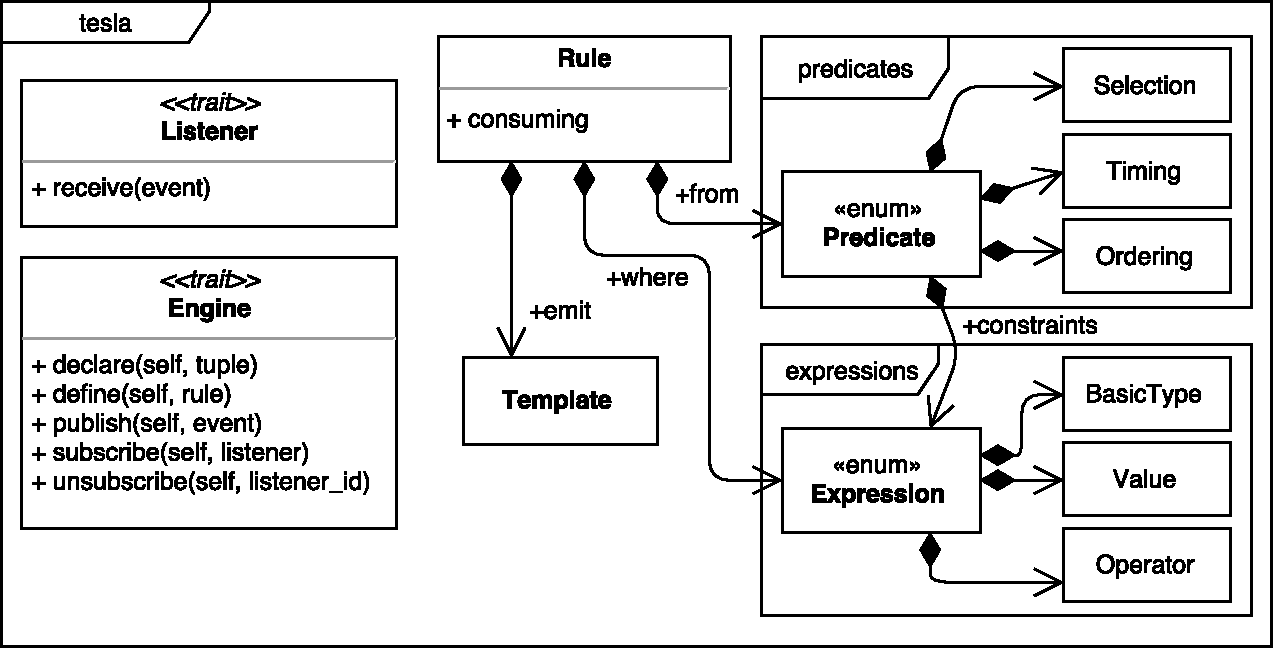
\includegraphics[width=\textwidth]{tesla_classes}
  \caption{Tesla crate overview}
\end{figure}

In tesla package I extracted all the aspects that aren't implementation related, so that it could work as minimal contact point between components like the library and the server. The core of the package is made of two traits: `Engine`, that defines methods for publish-subscribe, tuple declaration and rule definition, and `Subscriber`, that is used for event reception. Starting from these entry points the rest of the data structures just follows from the information required: in particular we have two sub-packages `predicates` and `expressions`, the first contains all the tools to describe patterns of events and static data, the latter contains the \emph{Abstract Sytax Tree} (AST) of algebraic and comparison expressions. They both heavily leverage rust native union type, giving them a terse design compared to the possible equivalent with C++ `variant`.

\subsection{TRex}

\begin{figure}[h]
  \centering
  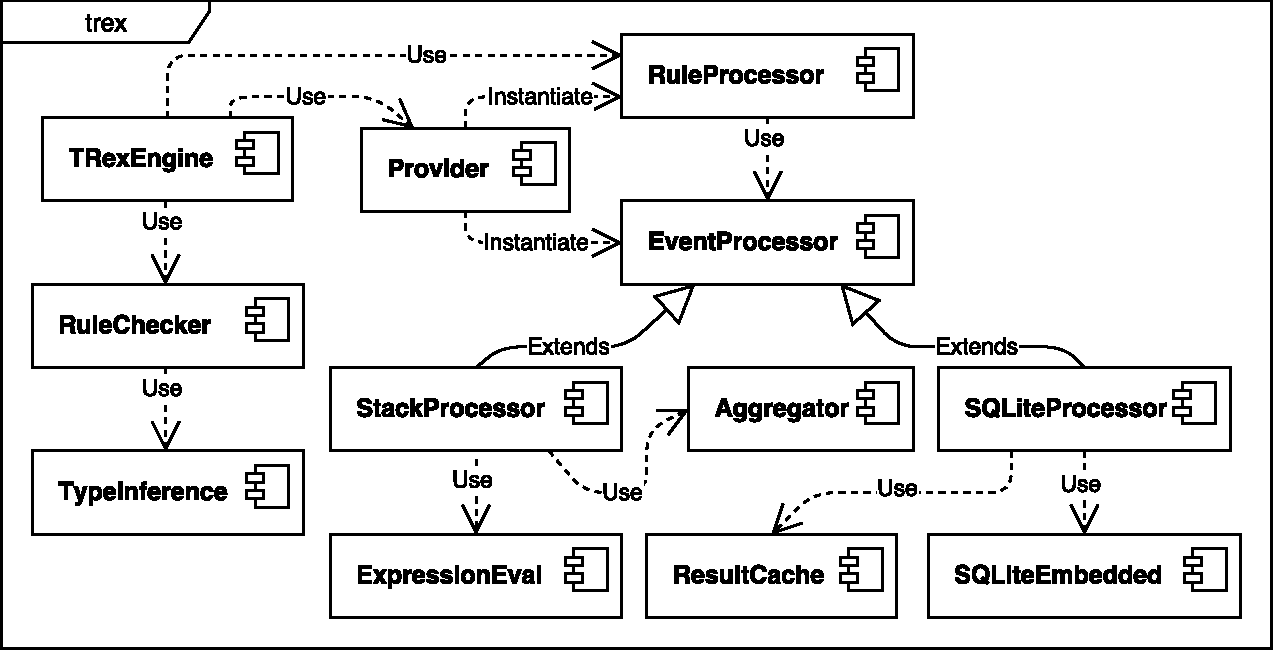
\includegraphics[width=\textwidth]{trex_components}
  \caption{TRex crate overview}
\end{figure}

The structure of `trex` crate closely recalls the previous implementation, with some simplification and new abstractions.

The core is the `TRex` struct, that implements the `Engine` trait and acts as a coordinator between the different components and the external world. The rest of the code can be divided in two main functionalities: the rule definition and the event processing.

The rule definition procedure is basically a sequence of configurations, that does not affect the performance of execution. When a new rule is received, `TRex` invokes the validation module and types, inferred from the collected tuple declarations, are checked to be used properly in expressions and assignments. If the rule passes the examination, a factory pattern is used to instantiate a dedicated `RuleProcessor`. Then the processor is indexed by the events that participate to the definition of the rule, so that is going to be activated only by those notifications that are relevant to its evaluation. In the original project the index was more sophisticated than a single hash-map and had a mechanism to filter the matches by checking those predicate constraints that only depend on immediate values. In practice the alternative appears to work well enough and additional optimization could be added if needed.

Event handling, instead, is the core of the business logic. Event notifications are sent to the `TRex` instance through the `publish` method, presented in pseudo-code in listing \ref{lst:publishmethod}. First the event is forwarded to the registered subscribers, then the index of rule processors is accessed and for each match a task is scheduled to execute in a thread pool, at this point the method is blocked waiting for tasks completion, finally if the evaluation does not produce new events the execution is complete otherwise the new events are submitted recursively to `publish` and the execution repeated. Since there is the assumption that incoming events are presented in time order and the blocking code prevent the next event from being processed, the time order for the generated complex events is guaranteed.\\
\begin{minipage}{\textwidth}
\begin{lstlisting}[caption={TRex publish method},label={lst:publishmethod},xleftmargin=.05\textwidth]
function publish(event):
  for_each subscriber in subscribers:
    subscriber.notify(event)
  done
  
  let processors = index.find_by(event.id)
  for_each processor in processors:
    thread_pool.execute { processor.process(event) }
  done
  
  let events = thread_pool.collect_results()
  for_each event in events:
  	self.publish(event)
  done
end
\end{lstlisting}
\end{minipage}\\
Going deeper, the `RuleProcessor`, which correspond to `StackRule` class in C++, is the coordinator of a sequence of `PredicatesProcessor` and its main method (in listing \ref{lst:processmethod}) is a generalized version of the Column-based Delayed Processing (CDP) algorithm that, as mentioned in chapter \ref{chap:tesla-trex}, is at the core of T-Rex library itself.\\
On event reception `RuleProcessor` is responsible of dispatching the notification to the predicates and, if the trigger is satisfied, of propagating the chain of evaluation. The evaluation is based on a list of objects called `PartialResult`, each them is a representation of sequence of tuples (events or static data) that are compatible with the pattern of predicates has been so far verified. Every step in the propagation consumes the list of partial results, filters it and enriches it with the predicate inner information, with the result that the list can be shrunk, expanded or dropped altogether. Once the evaluation is complete and successful, the `RuleProcessor` verifies the last constraints of the where clause and builds the events to emit from a template, possibly handling the consumption of some of the events used in the process.\\
\begin{minipage}{\textwidth}
\begin{lstlisting}[caption={RuleProcessor process method},label={lst:processmethod},xleftmargin=.05\textwidth]
function process(event) -> [event] :
  for_each predicate in predicates_processors:
    predicate.process(event)
  done

  results = []
  if trigger.is_satisfied(event):
    time = event.time;
    for_each predicate in predicates_processors:
      time = predicate.remove_old(time)
    done

    partial_results = []
    for_each predicate in predicates_processors:
      partial_results =
        predicate.evaluate(partial_results)
    done

    for_each partial_result in partial_results:
      if where_clause.is_satisfied(partial_result):
        results.push(template.fill_with(partial_result)
        mark_for_consumption(partial_result)
      fi
    done
  fi

  return results
end
\end{lstlisting}
\end{minipage}

In the previous version there were, clearly, only event based predicates and their different types (in term of event selection, aggregates and negations) were often coupled with business logic and in particular `StackRule` had to handle all of them explicitly, with specific functions and separate collections. T-Rex2 introduces a new abstraction, that is the aforementioned trait `PredicateProcessor` which is implemented by any component that acts as a predicate evaluator. In this way everything is handled uniformly: event and static processors are instantiated through a provider, for further decoupling, and kept into a unique list. Every time that a notification arrives all the elements of the list are notified and each of them decide how to handle the information. Similarly, during evaluation, the only mean of communication is through `PartialResult` and the nature of each step remains encapsulated.\\
This design choice makes it much easier to experiment with new data sources and hopefully this modularity will facilitate future development of custom components for different DBMS.

Currently the system runs two implementations of predicate processor: `EventProcessor`, which supports the previous functionalities and completes the CDP algorithm as in the original paper \cite{trex-cuda}, and `SQLiteProcessor`, that is the test implementation to interact with a relational database.\\
The `EventProcessor`, at every notification, filters the received event by ID and checking the constraint that depend only on immediate values, if everything matches the event is stored into a time ordered vector, which is periodically cleaned from old or consumed entries. When the evaluation starts and a `PartialResult` is received, the processor scans the events and propagates those that match every parameterized constraint.\\
The `SQLiteProcessor`, instead, doesn't interact with event notifications and it's activated only during the evaluation phase, when it queries the database to find suitable tuples, as we will see in the following section.

An example of rule processor is shown in figure \ref{fig:rule_processor}, where the rule is composed in sequence by a trigger, two event predicates and a static predicate. During the execution the two event processors have collected a stack of events, instead the SQLite processor has direct access to a DB table.

\begin{figure}[h]
  \centering
  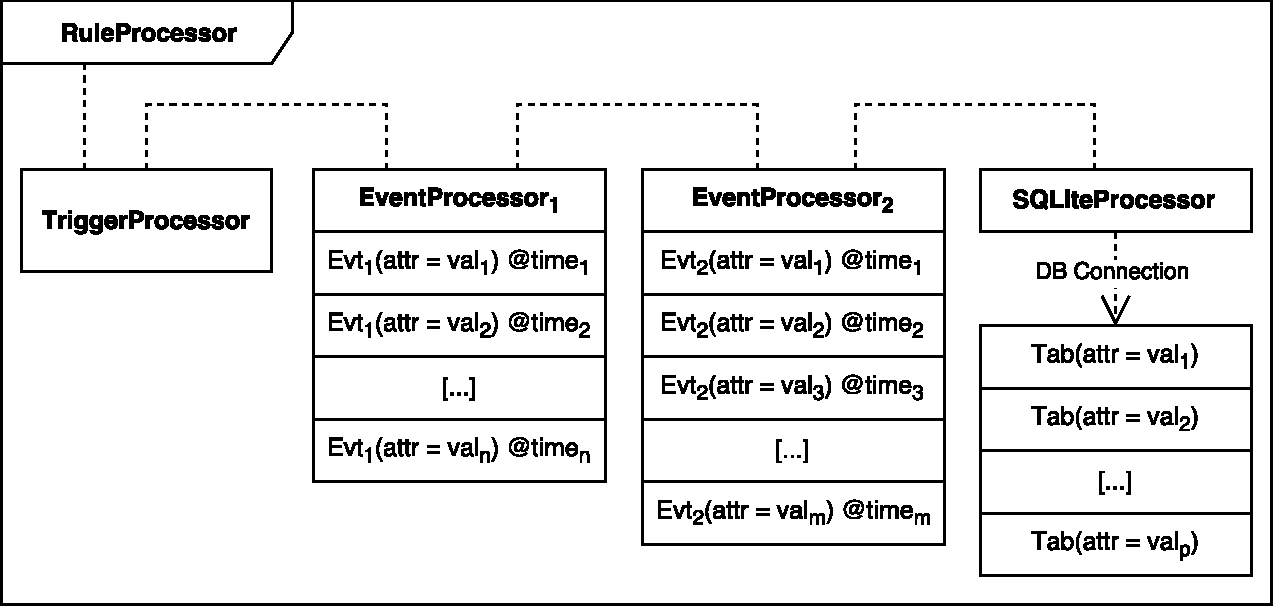
\includegraphics[width=\textwidth]{rule_processor}
  \caption{Processors chain example}
  \label{fig:rule_processor}
\end{figure}

\section{SQLite module}
The SQLite module contains two main components: a translator and an executor.

At creation time the predicate is fed to the translator and TESLA syntax is mapped permanently to a SQL statement using the following simple conversion rules.\\
The basic example is composed of an each predicate with no constraints nor parameters and, as we can see, the statement can be translated to a simple SQL select.
\begin{align*}% Example of each
&each\ SD\ \triangleq\\
&SELECT\ 1\ FROM\ SD;
\end{align*}
When the predicate features a negation, the operator `NOT EXIST` can be used to evaluate a subquery and return whether there are values in the result set or not.
\begin{align*}% Example of not
&not\ SD\ \triangleq\\
&SELECT\ NOT\ EXIST\ (SELECT\ 1\ FROM\ SD);
% For unexpected speed difference consider also:
% SELECT (SELECT id FROM SD) IS NULL;
% SELECT id FROM SD LIMIT 1;
\end{align*}
The selection policy $first$ does not have an implicit absolute ordering to work with, so it has to define one. The order clause is directly mapped to the SQL one.
\begin{align*}% Example of first
&first\ SD\ order\ by\ attr_1\ ASC,\ \ldots,\ attr_n\ DESC\ \triangleq\\
&SELECT\ id\ FROM\ SD\\
&ORDER\ BY\ attr_1\ ASC,\ \ldots,\ attr_n\ DESC\ LIMIT\ 1;
\end{align*}
For $last$ the same considerations made for $first$ hold, except for the mapping of the order clause, which is inverted.
\begin{align*}% Example of last
&last\ SD\ order\ by\ attr_1\ ASC,\ \ldots,\ attr_n\ DESC\ \triangleq\\
&SELECT\ id\ FROM\ SD\\
&ORDER\ BY\ attr_1\ DESC,\ \ldots,\ attr_n\ ASC\ LIMIT\ 1;
\end{align*}
The use of constraints inside tuple brackets find its correspondence in the SQL where clause.
\begin{align*}% Example of attribute constraint
&each\ SD(attr_1\ op \ val_1,\ \ldots,\ attr_n\ op \ val_n)\ \triangleq\\
&SELECT\ id\ FROM\ SD\\
&WHERE\ attr_1\ op\ val_1\ AND\ \ldots\ AND\ attr_n\ op\ val_n;
\end{align*}
The definition of a parameter it's processed adding its value to the query return column.
\begin{align*}% Example of parameter
&each\ SD[\$param = attr_i,\ \ldots]\ \triangleq\\
&SELECT\ attr_i\ as\ param,\ \ldots\ FROM\ SD;
\end{align*}
Finally the most common aggregation functions can be found in both the languages, so a translation is immediate.
\begin{align*}% Example of aggregates
&\$param\ =\ AGGR(SD.attr_1)\ \triangleq\\
&SELECT\ AGGR(attr_1)\ as\ param\ FROM\ SD
\end{align*}
The prepared statement produced is then stored for later use.

When the evaluation start, the executor populates the query with the parameters contained in `PartialResult` and execute it through `rusqulite` library (that is a wrapper of C SQLite embedded API) and the result are processed and forwarded in the chain of evaluation.

\section{Cache}
To improve performance of data retrieval and try to keep the speed of execution above the constraints of real-time, a caching layer was added between the executor and the database.
\begin{figure}[h]
  \centering
  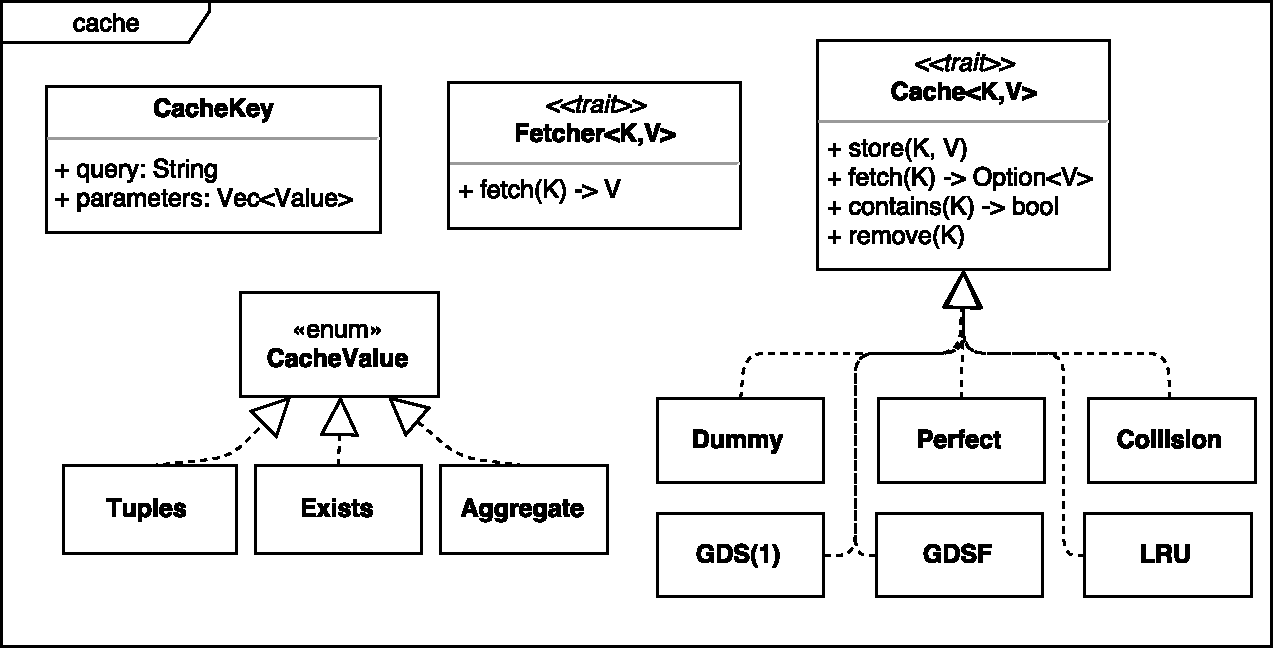
\includegraphics[width=\textwidth]{cache_classes}
  \caption{Cache module overview}
  \label{fig:cache_classes}
\end{figure}

The key of the cache is made by the combination of a SQL statement and the parameters with which it was populated. The key is intuitively unique for each result set\footnote{For the purpose of the thesis the data are considered immutable and cache invalidation is omitted} and it is also descriptive of the interrogation itself. So, instead of contacting the cache and database directly, the `SQLiteProcessor` will construct a key and delegate the task to a `Fetcher`. This new component will attempt a lookup in the cache and if the result is missing will fall back to the DB, hiding the complexity of cache update and multi-threaded synchronization.
The cache value is the result of a previously executed query and, depending from the type of the predicate, it can be a list of tuples or the result of an aggregate function or a flag of existence.

The system is integrated with several cache algorithms that can be activated and configured through the engine construction arguments.\\
Each of them, as can be seen in figure \ref{fig:cache_classes}, implements `Cache` trait allowing to easily replace one implementation with another.\\

\subsection{Simple Caches}
We can categorize the first three algorithm as simple caches, because they have basic storage approaches and do not leverage the context information to chose what to preserve and what to discard.
\paragraph{Dummy} The first implementation is a dummy cache that doesn't store anything and it's useful for testing the system in condition of 100\% misses. The methods `store` and `remove` are just empty, while `contains` will always return false and `fetch` will always `None`.
\paragraph{Perfect} The perfect cache is the opposite of the dummy and will store everything, without capacity limits. Its purpose is to test the maximum theoretical benefits of a cache. The methods simply forward the calls to those of an hashmap.
\paragraph{Collision} The collision cache is basically an hashmap with a reduced key space and a fixed capacity. The methods `contains`, `fetch` and `remove` act in the same way a normal map would. However the insertion possibly removes a single entry with the same hash value.\\

\subsection{Complex Caches}
The last three algorithms, instead, store metadata about the entries and exploit the context information to provide better chance to preserve useful entries in their limited available capacity.\\
\begin{minipage}{\textwidth}
\begin{lstlisting}[caption={Complex cache insertion},label={lst:complex-insertion},xleftmargin=.15\textwidth]
function store(key, entry):
  insert entry
  while memory usage > capacity
    remove the entry with least priority
  done
end
\end{lstlisting}
\end{minipage}\\
All the algorithms presented, as most of the caches in general, are characterized by an insertion method that operates, as shown in listing \ref{lst:complex-insertion}, by storing the new element to cache and removing the lowest priority element until the memory usage is below the allowed capacity. The difference between the three implementations is only the formula they use to compute priorities. All the other methods behave as in a standard map, except that `fetch` and `contains` function internally update the priority of the accessed element.

\paragraph{LRU-SIZE} \emph{Least Recently Used} is a family of caches that keep track of the order of access and prioritize time locality. In its usual implementation is meant for fixed size entries and, since in our case results sets can vary significantly in length we adopted the LRU-size variant. LRU-size has a maximum capacity set in terms of object sizes and, every time a value is inserted, multiple entries can be evicted to make room for the new one, keeping a controlled memory footprint. The cache was implemented on top of a `LinkedHashMap`, that is an hash map whose entries are connected one another in a linked list, having $O(1)$ complexity for each operation.

\paragraph{GDS(1)} \emph{Greedy-Dual Size(1)} \cite{gds1} is a cache developed in the context of web browsers and proxies. GDS(1) rewards small entries, so that in the same capacity will fit more values, increasing the probability of a hit. The priority is computed with the following formula:
\begin{align*}
priority\ :=\ 1\ /\ size\ +\ clock
\end{align*}
Where $clock$ is an aging factor to avoid stagnation of entries that aren't relevant anymore and it's updated monotonically as the priority value of the last discarded entry.

\paragraph{GDSF} \emph{Greedy-Dual Size Frequency} \cite{gdsf}, an evolution of GDS(1), is the current champion among the web caching algorithms and implemented, for example, by Squid caching proxy. It tries to consider a combination of how costly it is to obtain the entry, the size it occupies and the frequency it was accessed so far, with the following formula:
\begin{align*}
priority\ :=\ cost\ *\ frequency\ /\ size\ +\ clock
\end{align*}
Where $clock$ is the same aging factor seen for GDS(1).

Both GDS(1) and GDSF can be implemented using a expecially crafted combination of a binary heap and an hash map, with amortized $O(1)$ complexity and worst case of $O(log(N))$. However, for simplicity, it has been implemented using a high level combination of a B-tree set and an hash map, with complexity $O(log(N))$.


% TODO Results and performances
\chapter{Evaluation}

\section{Introduction}
CEP engines are used in a variety of scenarios, each of which has different requirements and settings, and that makes performance evaluation a true challenge. In fact there is not a universally agreed methodology of measurement and there are neither a reference workload, recorded from a real execution, nor a standard emulator, to generate a synthetic one.

The complexity is given by the high number of parameter that characterize the execution of the application and in particular by the different ways in which they interact.\\
In a real world scenario most of those variables are bound to the environment and very specific: the inputs are correlated one each other and together deliver a meaningful information, at the same time the rules are manually tailored to the particular task.\\
On the opposite side, during a general purpose evaluation, it is necessary to control the behavior of the inputs and the complexity of the rules, while preserving the stability of the execution.

In this chapter I will present the results of a selected number of test cases, explaining why each configuration was chosen and how it could impact on a real world application.

\section{Environment}
\begin{table}[h]
  \begin{center}
    \begin{tabular}{|c|c|}
      \hline
      Processor: 		& Intel Core i7-4770 @ 3.40GHz\\
                        & 4 Cores, 8 Threads\\ 
      \hline
      RAM size: 		& 16GB\\
      \hline
      Operating System: & Debian GNU/Linux 8.6 (jessie)\\
                        & Kernel 3.16.0-4-amd64\\
      \hline
      C++ Compiler:     & G++ 4.9.2\\
      \hline
      Rust Compiler:    & 1.14.0-nightly (2016-11-05)\\
      \hline
    \end{tabular}
    %\caption{Execution environment}
  \end{center}
\end{table}

\section{General Performances}
First of all, setting temporarily aside the introduction of static data, we will compare the previous T-Rex engine with the rewrite T-Rex2. This will show that the new implementation is indeed correct and efficient, mitigating the risk of a bias in the tests due to a poor realization. In the meantime we will gradually introduce the key points of the evaluation process and the general environment setup.

\subsection{Characteristic variables}
We start from the fundamental variables that characterize a CEP evaluation, in particular explaining their on the computation.
\begin{itemize}
\item The frequency of events and the size of predicate window are two of the most characteristic control variables and, in combination one with each other, they regulate the amount of events retained by the system. So higher frequencies and wider windows imply that more events will be associated with every predicate processor: those events have to be searched at each iteration of the system and directly concur in rules satisfaction.
\item The number of rules intuitively impact the computational requirements increasing the number of step needed to process an incoming event. However this aspect is strongly related with the number of declared event types and since the latter influence the probability of a rule being activated by the next random event. So a high number of rules composed by many different event types, may be activated just one at a time and stress the system way less than the half of the rules with fewer event declarations.
\item The number of predicates per rule and the presence of constraints on them influence the probability of a rule to be satisfied. In combination with the selection policy, measured in terms of probability of being $each$, $first$ or $last$, they determine how many new events will be generated by each rule.
\item Finally we mention the two most important output variables: the drop rate and the time of completion. The drop rate analyzes the system in a latency oriented fashion and it is measured as the percentage of discarded events: we feed the engine through a buffer queue of finite length and if it is not emptied fast enough the exceeding events are lost. On the other hand the completion time is more throughput oriented and it is obtained using an unbounded queue and waiting for the system to process every single event.
\end{itemize}

\subsection{Base rule}
As for the rule definition, the challenge is to create a model that is simple enough to predictably work under all the circumstances examined and rich enough to be interesting and customizable. We found the following rule to be representative of the different aspects we care about, while being easy to extend.
\begin{align*}
&declare\ SE_0(x:\ int)\ with\ id\ 0\\
&declare\ SE_1(x:\ int)\ with\ id\ 1\\
&declare\ \ldots\\
&declare\ SE_i(x:\ int)\ with\ id\ i\\
&declare\ CE()\ with\ id\ i+1
\end{align*}
\begin{align*}
&from\ SE_0(x == 1)\\
&and\ each\ SE_1(x == 1)\ within\ \tau_1\ from\ SE_0\\
&and\ \ldots\\
&and\ each\ SE_i(x == 1)\ within\ \tau_i\ from\ SE_{i-1}\\
&emit\ CE
\end{align*}

The rule is composed of a linear chain of simple events from $SE_0$ to $SE_i$, where every predicate has a temporal dependency with the previous one and the number of predicates can be extended at will. Each constraint is composed of a single equality to the immediate value 1, this configuration allows to simply control the match through the choice of event values. The time window is parameterized by $\tau_i$ and, while the example shows only the use of $each$ selection policy, they can be varied with a given probability.\\
Exactly $i+1$ tuples were declared, so that each one can only appear in a specific position in the rule, improving the predictability of the system.

\subsection{Workload}
\label{subsec:first-workload}
For the benchmark we configured the previous rule with $i=2$ and $\tau_i$ as a random random value uniformly distributed in the range $\tau_{avg} - 1s$ and $\tau_{avg} + 1s$.\\
The probability of choosing $each$, $first$ or $last$ selection policies was usually fixed to $100\%$ of $each$ to maximize the load of the system.\\
Regarding the rest of the system, $65$ group of $4$ event types were declared and $650$ rules were instantiated, $10$ identical for each group of events, so that every time a sequence was satisfied ten rules would fire. The events were generated uniformly across the different declarations, with all the attributes $x$ set to 1 to satisfy the constraints, and they were emitted at a tunable frequency. The number of events fed to the system was $60 * freq$, that is the quantity emitted in a minute at the given frequency. The length of the queue was bound as $freq / 10$ when measuring the drop rate and left unbound when measuring execution time.

\subsection{T-Rex and T-Rex2 comparison}
For the first comparison we set the predicates window to at an average of 10s and varied the frequencies from 600 to 4000 events per second, so that at the minimum both handle all the events, with a drop rate of 0\% and at the end of the scale most of them are lost.\\
Figure \ref{fig:trex_vs_rewrite_freq_drop} shows that the drop rate of the rewrite is lower at every frequency and similarly figure \ref{fig:trex_vs_rewrite_freq_time}, that plot execution times in second on logarithmic scale, shows that at frequencies where the engines would loose events the speed of the rewrite is almost constantly four times higher.
\begin{figure}[h]
\captionsetup{justification=centering}
\begin{minipage}{.5\textwidth}
  \centering
  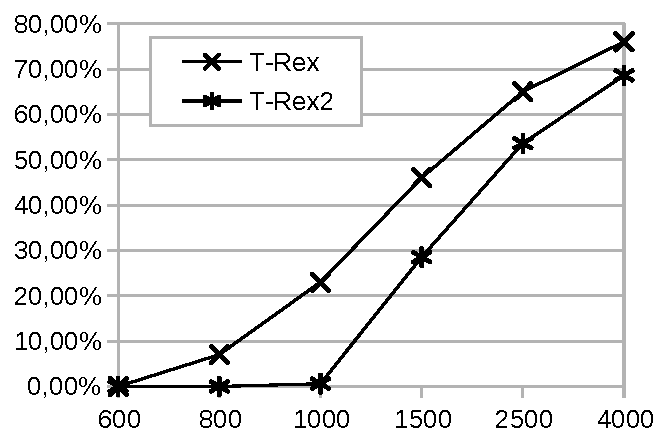
\includegraphics[width=.95\linewidth]{trex_vs_rewrite_freq_drop}
  \caption{T-Rex vs T-Rex2\\
  	Frequencies and drop}
  \label{fig:trex_vs_rewrite_freq_drop}
\end{minipage}%
\begin{minipage}{.5\textwidth}
  \centering
  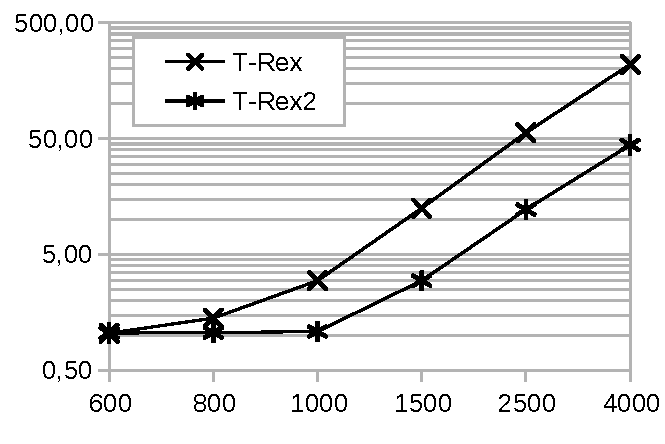
\includegraphics[width=.95\linewidth]{trex_vs_rewrite_freq_time}
  \caption{T-Rex vs T-Rex2\\
  	Frequencies and time}
  \label{fig:trex_vs_rewrite_freq_time}
\end{minipage}
\end{figure}

To better explore the domain, for the second comparison we pick a middle frequency, 1500, and vary the average windows size, in a range from 3 to 12 seconds.\\
The results, shown in figure \ref{fig:trex_vs_rewrite_win_drop} and \ref{fig:trex_vs_rewrite_win_time}, are noticeably similar to the first measurement and confirm the performance gain.\\
We can also observe how in both the test case the drop rate and the corresponding execution time are closely correlated and most of the time it is possible to switch from one to the other without loosing the qualitative interpretation.
% TODO maybe add the observation that
% they correlate exponentially: that is likely to happen since the system, discarding packages, reduces event retention and a 10\% global reduction, translates in a 10\% at each step of the pattern composition
\begin{figure}[h]
\captionsetup{justification=centering}
\begin{minipage}{.5\textwidth}
  \centering
  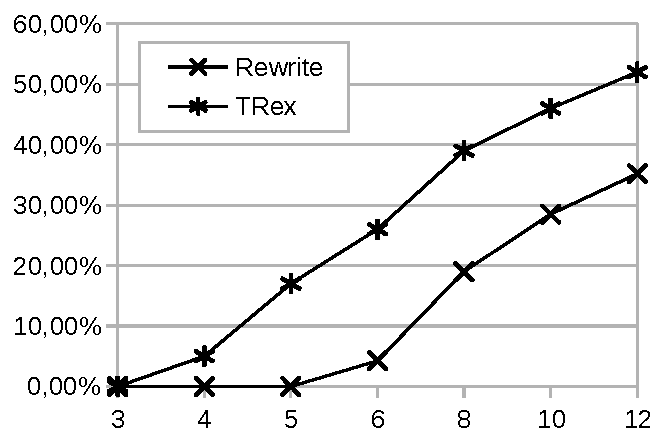
\includegraphics[width=.95\linewidth]{trex_vs_rewrite_win_drop}
  \caption{T-Rex vs T-Rex2\\
  	Windows and drop}
  \label{fig:trex_vs_rewrite_win_drop}
\end{minipage}%
\begin{minipage}{.5\textwidth}
  \centering
  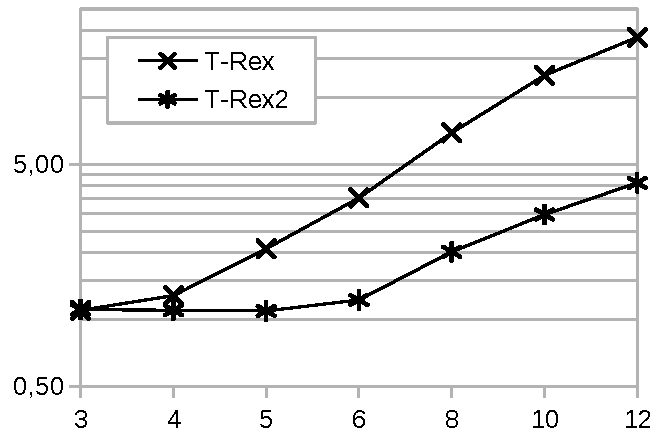
\includegraphics[width=.95\linewidth]{trex_vs_rewrite_win_time}
  \caption{T-Rex vs T-Rex2\\
  	Windows and time}
  \label{fig:trex_vs_rewrite_win_time}
\end{minipage}
\end{figure}

The results demonstrate the efficiency of T-Rex2, with improvements that can be considered beyond the expectations, considering that the rewrite closely followed the architecture of its predecessor. The most likely and relevant motivation is a slightly improved parallelism that take advantage of all the available processing units: they both had 8 workers threads (plus few other to deal with coordination and event publishing), but the old implementation distribute the jobs statically using rule ids, while the rewrite allocate them dynamically with a thread pool.\\

\section{Static data and Cache}
In this section we are going to explain how the execution must be adapted to evaluate the interaction between events and persistent data and to test the performance gains obtained from the cache.

\subsection{Additional variables}
We must refine the domain of the problem, since the new expressivity inevitably causes the expansion of the control variables with the one needed to describe the properties of the database and the cache layer.\\
In particular a database is a complex technology and have plenty of settings and characteristic, but the fundamental ones are: the number of rows, the number of columns, the distribution of the values, the latency of the connection and the presence of indexes. While the integration into the CEP execution is characterized by the selection policy, the constraints on the values, the number of results and the frequency of invocation.\\
As for the cache, there is the choice of the algorithm among the many presented, the size in terms of memory occupation and finally the possibility to share the storage or split it among the different users. Moreover there are environmental factors that influence the results like the domain and the probabilistic distribution of the values. Finally miss rate and hit and miss time are the characteristic metrics of performance.

\subsection{Rule adaptation}
The previous TESLA rule was kept as a template and extended with a static predicate with the following configuration:
\begin{align*}
&declare\ SE_0(x:\ int)\ with\ id\ 0\\
&declare\ SE_1(x:\ int)\ with\ id\ 1\\
&declare\ \ldots\\
&declare\ SE_i(x:\ int,\ y:\ int,\ z:\ int)\ with\ id\ i\\
&declare\ SE_{i+1}(col_0:\ int,\ \ldots,\ col_j:\ int)\ with\ id\ i+1\\
&declare\ fact\ SD(col_0:\ int,\ \ldots,\ col_j:\ int)\ with\ id\ i+2\\
&declare\ CE()\ with\ id\ i+3
\end{align*}
\begin{align*}
&from\ SE_0(x == 1)\\
&and\ each\ SE_1(x == 1)\ within\ \tau_1\ from\ SE_0\\
&and\ \ldots\\
&and\ each\ SE_i[\$p_1 = y,\ \$p_2 = z](x == 1)\ within\ \tau_i\ from\ SE_{i-1}\\
&and\ each\ SD[\$c_0 = col_0](col_1 >= \$p_1,\ col_1 < \$p_2)\\
&emit\ CE(x = \$c_0)
\end{align*}
There is a new declaration $SD$ that describes the static data collection and each of its attributes is mapped to a column of the table.\\
The event $SE_i$ acquire a special role, it has a second and third attribute, that are referenced in the static predicate and they work as lower and upper bound, controlling the result of the query.\\
Another declaration was introduced, $SE_{i+1}$, that, as we will see, can be used as a replacement of $SD$ whenever we want to reduce the access to the DB while keeping the same level of produced events.\\
Finally it is possible, through a configuration, to add a parametric dependency between the static predicate and other predicates in the rule: this allow to expand the domain of the cache key stressing the cache algorithms.

\subsection{Workload}
\label{sec:second-workload}
% database creation, database random data, extension of the rule (last predicate), 1000 rules 100 declarations, highly frequent and dense, now focused on each sel policy
First of all, a database table is created with 2 columns (an incremental index and a numerical payload) and populated with a given number of rows. In particular, for each entry the aforementioned payload is randomly generated in a range between $-1 / 2 * \#rows$ and $+1 / 2 * \#rows$: having a uniform distribution of values, but in a non sequential order, helps to avoid possible bias in term of DBMS architecture or file read.\\
The declaration were changed to 100 groups of 5, plus one single declaration for the database table. The rule defined are 1000, preserving the ratio of 10 identical rule for each declaration group. Database indexing can be switched on or off.\\
During the event generation, $SE_i.y$ (the second attribute of the events of type $SE_i$) is set to a random value, sampled from a selectable probabilistic distribution, while $SE_i.z$ is set as $SE_i.y + \Delta$, so that they act properly as lower and upper bound. Where $\Delta$ is generated pseudo-randomly with an average of 10.\\
What is not mentioned here is unchanged from the previous definition of the workload in section \ref{subsec:first-workload}.

\subsection{Table simulation and database}
Even without a native support for DBMSs, it was already possible to emulate the access to a persistent data collection, as we recall from section \ref{sec:intro-lang-extension}. So it seems appropriate to verify the integration with SQLite to be consistently faster than preexisting alternative.

So, to define two executions with the very same semantic, we applied the algorithm for DB population to produce events with the same payload of the corresponding table and we emitted all of them at the beginning of the execution. At the same time we adapted the static predicate in each rule extract the same data from the simulated event stream (using an unlimited window, to have the data available at any time).

\begin{figure}[h]
  \centering
  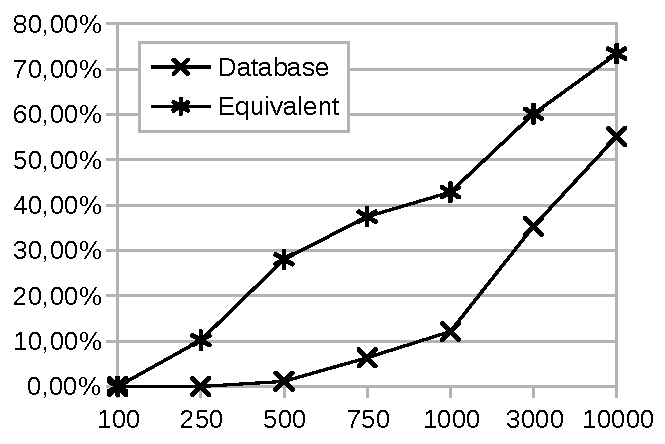
\includegraphics[width=.6\textwidth]{equiv_vs_db_800r_drop}
  \caption{Database vs simulation}
  \label{fig:equiv_vs_db_800r_drop}
\end{figure}

We execute the programs with a small window of 2s average and low frequency of 800 events per second, varying the number of static data entries from 100 to 10000. As we can see from figure \ref{fig:equiv_vs_db_800r_drop}, the table simulation fully handle the load only with a very small collection and performances rapidly deteriorate as soon the number of static entries grow. On the other hand, T-Rex2 does not lose events even with the highest configuration considered. It is worth noting that, actually, thanks to the benefits of the database index, the performance of T-Rex2 are virtually not influenced by the size of the table (tested up to 10 million rows).
% TODO add second test with high performances

The results show that a native support is clearly an important improvement to the previous possibilities, but at the same time they give us little information about the limits of T-Rex2.

\subsection{Performances contextualization}
In the following benchmark we contextualize the measures collected through a comparison of the results of three different configuration that have the same rate of event production, meaning that given the same number of input events they will output a similar number of complex events.\\
Two out of thee different competitors share exactly the same workload described in section \ref{sec:second-workload}, one uses the dummy cache and the other uses the perfect one. The remaining execution does not have static predicates and is constructed in this way: each predicate of type $SD$ is replaced with one of type $SE_{i+1}$, with no constraints and unlimited window, and then events of type $SE_{i+1}$ are generated in the same number as the average length of the database result set (10 in this case). In this way the behavior of the system is closely simulated.\\
The test is run with an average predicate window of 6 seconds, 1 million of table rows (where used) and a frequency of events that vary from 600 to 4000 events per second.

\begin{figure}[h]
  \centering
  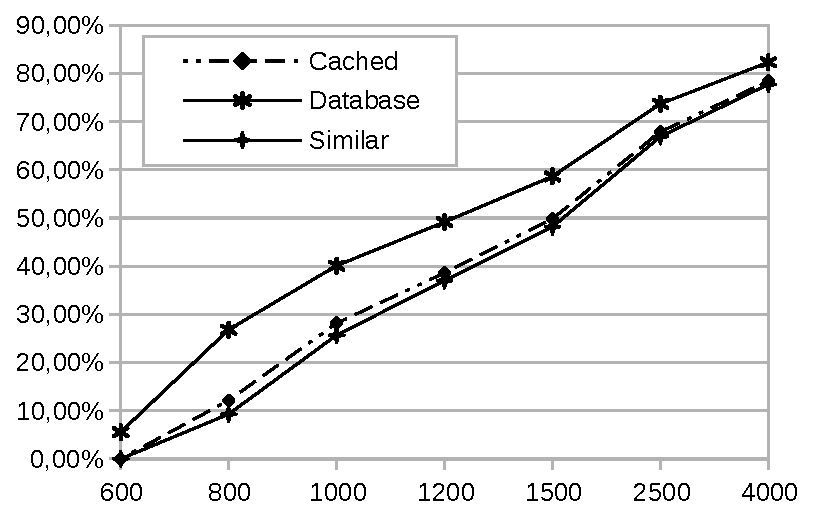
\includegraphics[width=.85\textwidth]{db_or_not_db_cached_drop}
  \caption{Perfect cache - Frequency and Drop}
  \label{fig:db_or_not_db_cached_drop}
\end{figure}

The results in figure \ref{fig:db_or_not_db_cached_drop} shows that that T-Rex2 integrated with SQLite in combination with a perfect cache (dashed line in the middle) can almost keep up with an execution that does not require access to the database (lowest line), loosing just around $2\%$ of events more than the competitor. At the same time the execution with the dummy cache draw a lower limit for the worst case performance: so, even in presence of non cache-friendly data or using less performing caches, the system is still capable of handling a remarkable load, likely enough to satisfy the requirements of many real applications.

\subsection{Cache algorithms}
% LRU_SIZE vs GDFS vs COLLISION (not a big difference, why?)
Now that we have defined some term of comparison and showed the results of the best and worst cache, in the following paragraphs we are going to analyze the performance of all the cache algorithms presented in section \ref{sec:cache-impl} to see how they compare one with the others.

For the execution we set a frequency of 2000 event per second and 2 seconds window, with the event payload sampled from a normal distribution $\mathcal{N}(\mu = 0,\ \sigma = 30)$ and making the static query dependent from the last two predicates (expanding the query parameterization space, making harder to cache enough values). Then we vary the cache size, measured as the number of the rows contained in each cache object, from 500 to 6000.\\
We first analyze the miss rate of each algorithm, see figure \ref{fig:cache_showdown_miss}, and then compare it to the corresponding drop rate to evaluate the impact on the global execution, see figure \ref{fig:cache_showdown_drop}.

\begin{figure}[h]
  \centering
  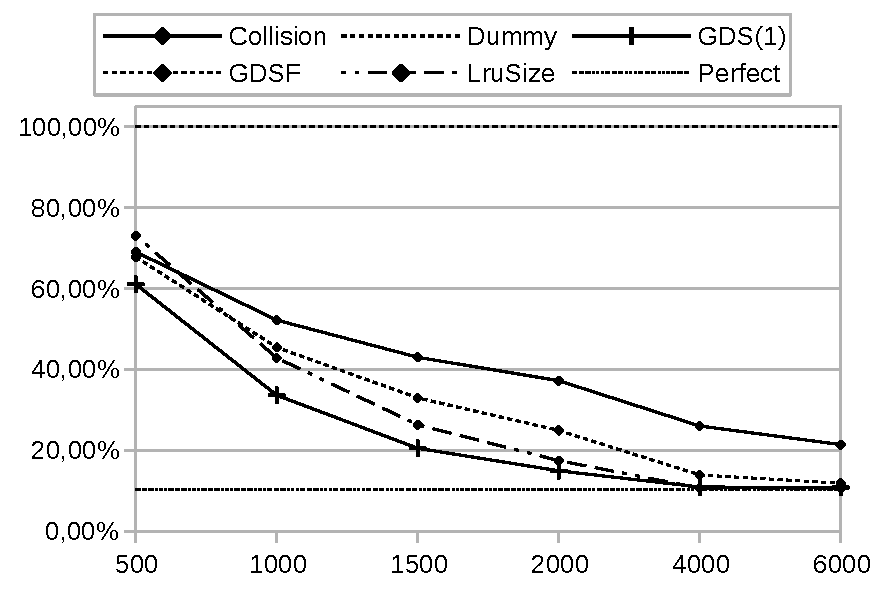
\includegraphics[width=.8\textwidth]{cache_showdown_miss}
  \caption{Cache comparison - Frequency and Miss}
  \label{fig:cache_showdown_miss}
\end{figure}
\begin{figure}[h]
  \centering
  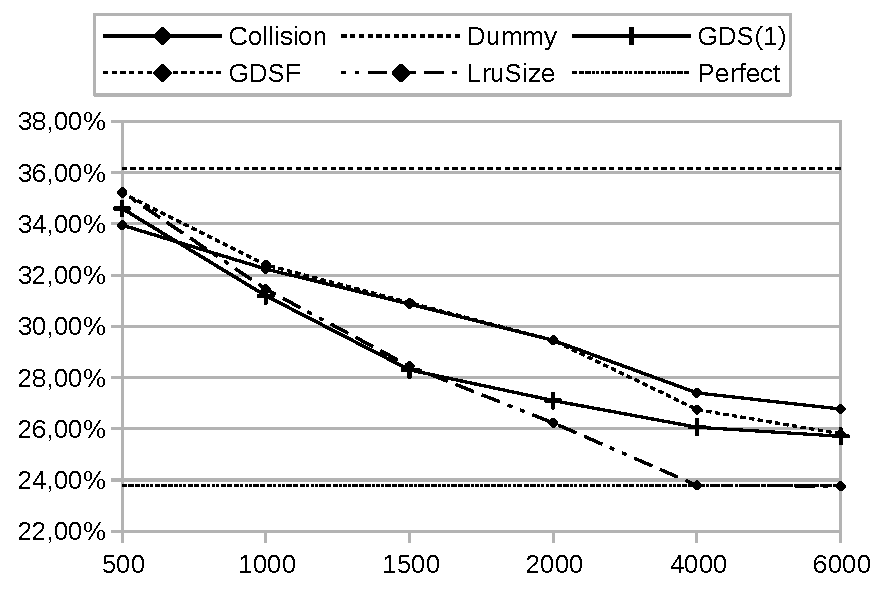
\includegraphics[width=.8\textwidth]{cache_showdown_drop}
  \caption{Cache comparison - Frequency and Drop}
  \label{fig:cache_showdown_drop}
\end{figure}

The dummy cache once again shows the worst case performances with $100\%$ miss rate. While the perfect cache sets the upper limit for the maximum efficiency achievable, with a $10\%$ of miss rate. They are shown on the charts as a horizontal line respectively at the top and at the bottom of the plots. At the end of the execution the perfect cache contained about 12000 entries, that is the size of the key space.\\
The collision cache, that is built on a very basic replacement policy, had a poor performance and was exceeded by every other algorithm.\\
However it was unexpected to see the GDSF cache, that is the de facto standard and champion in HTTP caching, to be clearly left behind in the comparison. My intuition is that its measure of frequency does not work well with the repeated access patterns of a CEP engine would require a more precise tuning.\\
The second best is the LRU-size, that proves itself to be a good allround solution and the first choice for any caching purpose. The winner of the comparison is the GDS(1) cache, that choosing smaller entries is able to maximize the memory usage. We can also notice, that both the top two algorithms reach the level of optimality of the perfect cache with a size between 2000 and 4000 entries, that means 3 to 6 time less than the actual key space.

Comparing the results with the plot of system wide performances, we show that the sole minimization of the miss rate it is not sufficient affect the global execution. The most notable example is how GDS(1), champion of the previous category, fails to keep up with LRU. The phenomenon is explained by the difference in term of hit time: in fact GDS(1) does have more hits (between $5\%$ and $10\%$ more), but with a cost of almost the double of the LRU ($\sim 1200 \nu s$ compared to $\sim 650 \nu s$ of access time). The reason behind this slow down is likely due to the suboptimal GDS(1) implementation.

\subsection{Shared or per predicate}
When the cache is allocated as a single storage accessed by different predicates, if they request similar data they will share the space and the cache loading cost. Also if there is some process that has more benefits from caching, an advanced algorithm could reward it with more space in memory. However there is always the risk that a single component would hog the entire space, filling it with garbage and degrading the system wide performance.\\
A cache per predicate, instead, would be much smaller, but it could better adapt to the specific pattern or distribution of the data.\\
However we found out to be another the most relevant factor decision: sharing the cache across multiple threads require constant synchronization. In the implementation the cache is wrapped with a mutex that soon became the bottleneck of the entire parallelization.

\subsection{Data distribution}
First of all we need to clarify that having a discrete and not too dense domain of values is a fundamental requirement, otherwise even in the smallest range there would be to many elements to hope for a reasonable match in the cache. So for example floating point numbers usually not adapt to take part to the cache key.\\
The effectiveness of a cache is based on assumptions on the processed data, for example time locality, meaning that a value requested recently is likely to be requested again. Each assumption may fit better or worse depending from the actual data distribution.

The system was built to offer a choice about the distribution of the input event values. So it is possible to experimented with gaussian, exponential and uniform distributions tuning the parameters to spread or narrow the range of the samples.\\
However we found out that this is only partially relevant, in fact there is a limit to the variability that can be introduced by a single event: because of the nature of the system, only a restricted number of events is queued in a processor and that is the maximum expression of the distribution. Conversely sequences of evaluation are executed repeatedly and the same data is requested many time during a single system iteration, so the benefit of the cache prevail over any possible distribution.\\
The situation changes when we make the static predicate dependent from more than one event at a time: in this case the probability distributions combine with each other and generate a wider and more diverse output, challenging the capacity of the cache.

%\section{Additional factors}
%\subsection{Event selection policy}
% EACH vs FIRST/LAST
%\subsection{Percentage of static predicates}
% PERCENTAGE OF STATIC PREDICATES and SATURATION FREQUENCY
%\subsection{Parallelism}
% N OF CORES


% Conclusions
\chapter*{Conclusions}
\addcontentsline{toc}{chapter}{\tocEntry{Conclusions}}
\markboth{CONCLUSIONS}{}

% TODO state of the art? (spark? flink? esper?)

In this dissertation we presented an extension to the TESLA language to describe the interaction between persistent data collection and event streams, showing that is possible to obtain a powerful abstraction without loosing the simplicity of the declarative language and preserving the formal definition of its operators.

We showed how, with an embedded database, its possible to handle millions of rows within the strict latency requirements of a real-time software and how, in presence of discrete and recurring data, the use of a cache can bring the performances almost on par with those of an equivalent load of pure events. In particular we demonstrated that the integration developed outperforms the workarounds that were previously needed to emulate the functionality.

However we verified that the attached source of data has to reliably respond within acceptable time constraints, otherwise not even the best cache can compensate for the slowdown. The problem is emphasized by the guaranties of time order execution enforced with a blocking architecture: this has been found to be a risky point of failure, because a delay of even a single call to the database may cause the system to stall. So for future development we suggest the investigation of a fine grained model of concurrency, the possibility to configure the desired level of guaranties and a integrated mechanism of error handling.

We also observed that the language allows multiple formulation of equivalent rules which may produce different execution plans, at the moment the responsibility to choose the most efficient alternative is left to the programmer, but this task could be automated introducing a step of rule rewriting.

In conclusion we think that the extension was a successful example of the proposed interoperabiliy and it is worth refining and expanding with new adapters. However it introduced many changes to the project and in the immediate future there will be a period of stabilization and reintegration of all the existing components, like the parser and the gpu processor.

\addcontentsline{toc}{chapter}{\tocEntry{Bibliography}}
\markboth{BIBLIOGRAPHY}{}

\printbibliography

\end{document}
